\documentclass[a4paper, 12pt]{article}
\usepackage{tikz}
\usetikzlibrary{arrows.meta}
\usetikzlibrary{automata}

\newcommand{\NodeLabel}[1]{\node(#1){$#1$};}

\begin{document}
\begin{figure}[h]
  \centering
  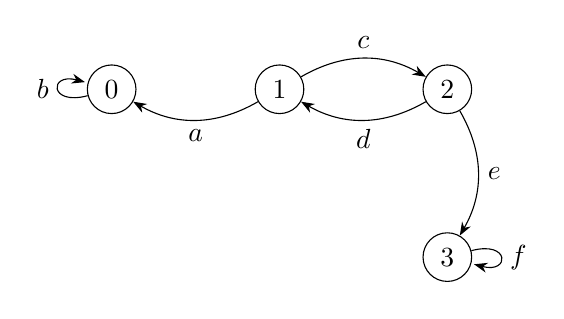
\begin{tikzpicture}[
    >=Stealth,
    auto
    ]

    \matrix[
    column sep=1.5cm,
    row sep=1.5cm,
    nodes={draw, circle},
    ]{
      \NodeLabel{0} & \NodeLabel{1} & \NodeLabel{2}\\
      &&\NodeLabel{3}\\
    };

    \path[
    ->,
    ]
    (2) edge[bend left]  node{$d$} (1)
        edge[bend left]  node{$e$} (3)
    (1) edge[bend left]  node{$c$} (2)
        edge[bend left]  node{$a$} (0)
    (0) edge[loop left]  node{$b$} (0)
    (3) edge[loop right] node{$f$} (3);

  \end{tikzpicture}
\end{figure}


\end{document}
